% !TEX root = ../../Thesis_main.tex
\section{Objectives and Motivations}

The goal of this work to improve methods of 3D reconstruction in holistic context using deep learning systems. For efficient applications such as robotics in human environments and mixed reality more advanced machine perception systems are needed. Human perception is a complex system with several properties not all of which are replicated in modern machine perception systems. From cognitive sciences it's known that ability to model environments is one of the most important for perception system, in area of computer vision this is known as an ability to perform \textit{3D reconstruction} of scenes and environments as shown on Fig~\ref{fig:holistic_reconstruction}. To solve this problem in a general case requires application of machine learning.

\begin{figure}
	\centering
    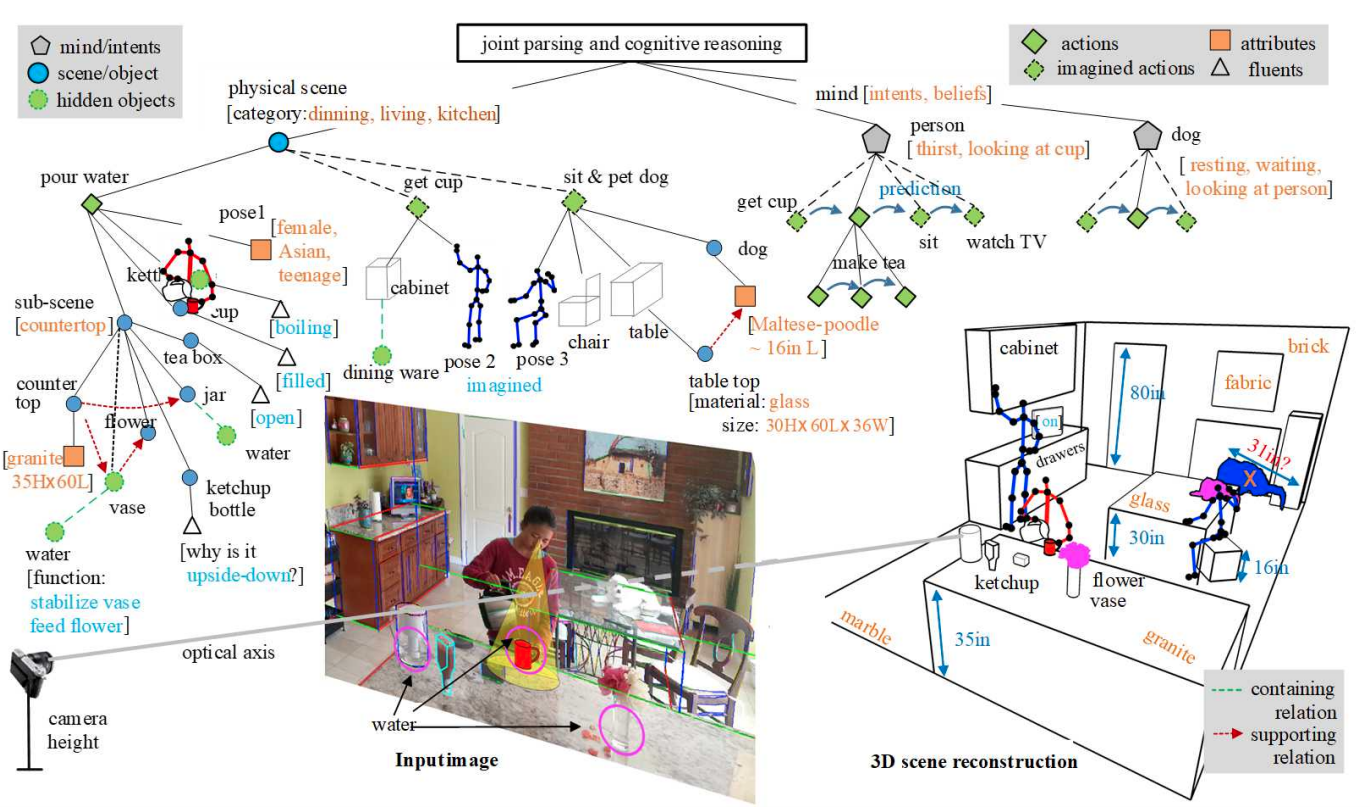
\includegraphics[width=\textwidth]{Figures/holistic_scene_reconstruction.png}
    \caption{An example of a holistic scene understanding or an image parsing. From a single image or a collection of different kinds of images regestered by various sensors, a computer perception system should be able to simultaniously reconstruct the 3D scene, estimate objects, their materials and shape, find correspondig records in an object database and parse scene hierarchically for unknown objects constructed from known parts. source: \cite{zhu2020dark}}
    \label{fig:holistic_reconstruction}
\end{figure}

In particular, the development of such holistic deep 3D reconstruction system includes several important tasks:

\begin{itemize}
    \item Capturing scenes, complete with colour and depth data of a sufficient quality,
    \item Segmenting variety of elements from sensor data, such as most common household objects and architectural components (e.g. floor, walls, ceiling, windows and doors),
    \item Recalling objects from large scale database of objects,
    \item Detecting and reconstructing shape and pose of the human bodies.
\end{itemize}

Each of these sub-tasks constitutes a challenge in the context of human perception.

Having a system that can parse indoor scenes with variable amount of objects with labels and get representations of unknown objects are natural needs for augmented/virtual reality applications and robotics.

\subsection{Overcoming noise in depth images}
The presence of noise in sensor data (e.g., consumer grade depth cameras) is a serious problem for all downstream sub-tasks, low fidelity of this data causes a considerable compaunding performance drop. Results obtained in \chapt{depth_superresolution} specifically targeted at quality improvement of these depth images.

\subsection{Shape retrieval}

Indoor environemnts mostly populated by human made objects with regular shapes and appearance determined by design and materials used, therefore they have a high amount of redundancy wich can be levered for retrieval purposes. Using Sparse 3D CNNs allows us to compute features which represent these objects and enable us to find them in a shape database. 

\subsection{Body Shape Reconstruction}

\textit{Body Shape Reconstruction} also known as \textit{Body Shape Regression} is a task often jointly approached with pose reconstruction.


% \begin{figure}
%   \begin{subfigure}{0.45\textwidth}
%     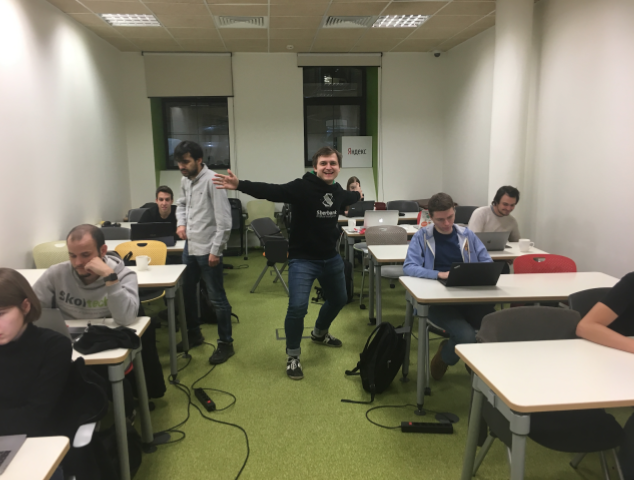
\includegraphics[width=\linewidth]{Figures/orig_densepose}
%     \caption{original image} \label{fig:orig}
%   \end{subfigure}%
%   \hspace*{\fill}   % maximize separation between the subfigures
%   \begin{subfigure}{0.45\textwidth}
%     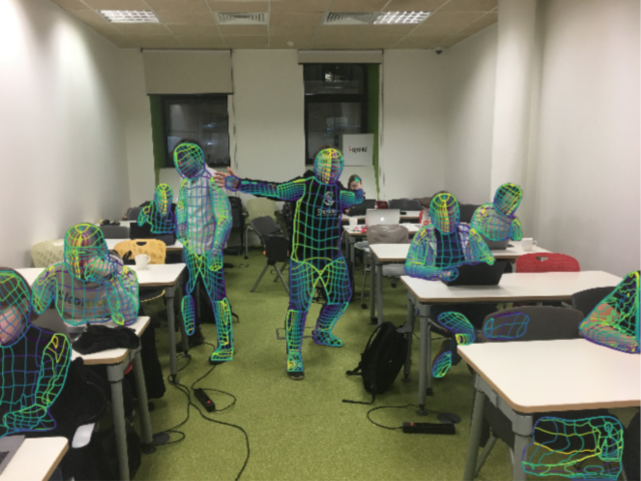
\includegraphics[width=\linewidth]{Figures/proc_densepose}
%     \caption{3D surface meshes overinposed in original image} \label{fig:proc}
%   \end{subfigure}%
% % \caption{A figure that contains three subfigures} \label{fig:1}
% \end{figure}


\begin{figure}[!tbp]
% \vspace{-20pt}
\centering
\begin{minipage}[b]{0.45\textwidth}
  \centering
  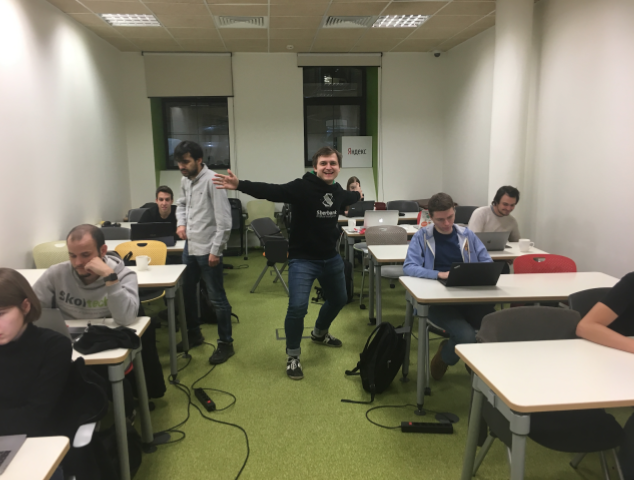
\includegraphics[width=\columnwidth]{Figures/orig_densepose}
  \caption{original image}
  \label{fig:orig}
\end{minipage}
\begin{minipage}[b]{0.45\textwidth}
  \centering
  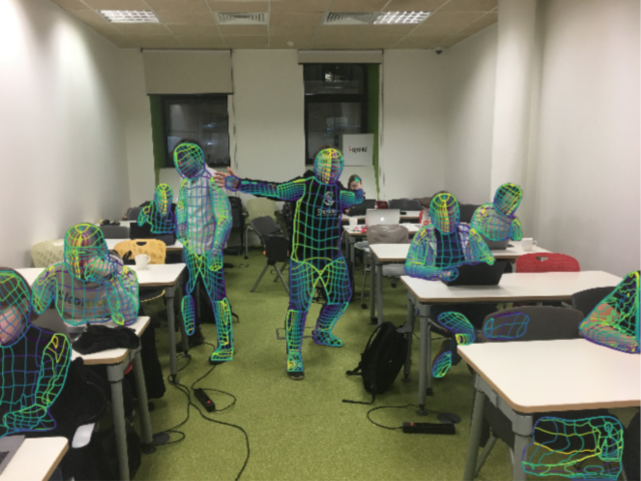
\includegraphics[width=\columnwidth]{Figures/proc_densepose}
  \caption{3D surface meshes}
  \label{fig:proc}
\end{minipage}
\end{figure}


DensePose-COCO dataset contains a large set of images of people collected ``in the wild'' together with different annotations: (i) bounding boxes, (ii) foreground-background masks, (iii) dense correspondences --- points $p \in S$ of a reference 3D model $S\in\mathbb{R}^3$ of the object associated with triplets $(c, u, v) \in\{1, \ldots, C\} \times[0,1]^{2}$, where $c$ indicates which one of $C$ body parts contains the pixel and $(u,v)$ represents the corresponding location (UV coordinates) in the chart of the part \cite{smpl}.
The DensePose task is then to predict such triplets $(c, u, v)$ for each foreground pixel and every person in the image.

The baseline dense pose prediction model, and all the subsequent works \cite{parsing, uncertainty, monkeys} follow the architecture design of Mask R-CNN \cite{maskrcnn}.

The model is a two-stage: first, it generates class-independent region proposals (boxes), then classifies and refines them using the box/class head. Finally, the DensePose head predicts the body part and UV coordinates for each pixel inside the box. Particularly, the model consists of many different blocks (see Fig.~\ref{fig:scheme}):
\begin{itemize}
    \item \textit{Backbone} to extract features from the image,
    \item \textit{Neck} to integrate features from different feature levels of the backbone to effectively perform multi-scale detection,
    \item \textit{Region proposal network (RPN)} to propose a sparse set of box candidates potentially containing objects,
    \item \textit{Heads} take the features pooled from the bounding box on the corresponding feature level, where the detection occurred, and produce output. The first head is a box/class head, which finally predicts whether the object is present in the box and refines the box coordinates. The second head is the DensePose head that predicts either the pixel belongs to the background or assigns it to one of the 24 DensePose charts, and regresses UV coordinates to each foreground pixel inside the bounding box.
\end{itemize}

\subsection{Hierarchical Scene Segmentation}

%Motivation: RGB-D scanning is here and we want to have a fine-grained understanding of the 3D captures
In the recent years, a wide variety of consumer-grade RGB-D sensors, such as the Intel Real Sense, Microsoft Kinect, depth-sensor enabled smartphones, enabled inexpensive and rapid RGB-D data acquisition. Increasing availability of large, labeled datasets (e.g.,~\cite{chang2017matterport3d,dai2017scannet})  made possible development of deep learning methods for 3D object classification and semantic segmentation. At the same time, acquired 3D data is often incomplete and noisy; while one can identify and segment the objects in the scene, reconstructing high-quality geometry of objects remains a challenging problem.  

An example of the new approach in recent work 
\cite{avetisyan2019scan2cad}, uses a large dataset of clean, labeled geometric shapes
\cite{chang2015shapenet}, for classification/segmentation associating the input point or voxel data with object labels from the dataset, along with adapting geometry to 3D data.  This approach ensures that the output geometry has high quality, and is robust with respect to noise and missing data in the input.  
At the same time, a ``flat'' classification/segmentation approach, with each object in the database corresponding to a separate label and matched to a subpart of the input data corresponding to the whole object, does not scale well as the number of classes grows and often runs into difficulties in the cases of extreme occlusion (only a relatively small part of an object is visible). 
Significant improvements can be achieved by considering object \emph{parts}, or more generally part hierarchies. 
Part-based segmentation of 3D datasets promises to offer a significant improvement both in finding the best matching shape in the dataset, recognizing objects from  highly incomplete data (e.g., from a couple of parts) from  as well as more precise geometry adaptation as well as, potentially, assembly of new shapes out of existing parts yielding a closer match to the input data. 

large collection of 3D models in database can be reduced to structured representations, 
objects with occluded sub-parts still can be recognized by parts available in the scan and the rest can be guessed with high probability, using parts, we can reconstruct new objects that are not yet present in the database of shapes.

Based on different approaches for volumetric information integration, from enhancements of  methods such as volumetric fusion \cite{curless1996volumetric}, to probabilistic  methods, and plethora of methods based on their combinations.

Compared to computer graphics models manually created by 3D professionals, 3D scans are noisy and incomplete.
Amount of noise and limited resolution of consumer-grade scanning hardware pose significant challenges for solving this important problem of scene reconstruction. 
Approaches of reconstruction based on fitting existing 3D assets into scene scans, have shown a lot of promise but still had problems with finding exact models from large database such as ShapeNet \cite{chang2015shapenet}, because of occlusion and lack of spatial context.

Learning-based approaches are very good at extracting features representative of objects and scenes as a whole, allowing to fill in occluded areas or guess parts affected by noise \cite{dai2017shape,dai2018scancomplete,song2017semantic}. These features are sufficient for scene completion, but they are not as good at recovering geometric primitives like: sharp edges, planar surfaces or borders between sub-parts, resulting in reconstruction quality much poorer than that of 3D content created by humans.

In this work, we focus on the key problem of semantic part segmentation of objects in the scenes, enabling further improvements in  dataset-based reconstruction. 
Semantic part-segmentation, can help in these situations, when sufficient number of the object parts is visible model can infer the non-visible parts essentially completing an object in sense of maximum probability conditioned on input data.

In human-made environments, a lot of objects have naturally defined semantic sub-parts, and those sub-parts can, in turn, have their sub-parts, i.e., parts form \emph{hierarchies}.  In our work, we use scene and object representation based on such part hierarchies.  We show how a part-labeled dataset of scanned 3D data suitable for machine learning applications can be constructed, and used to improve the performance of segmentation algorithms. 

Definitions of sub-parts are based on a set of primitive elements that were manufactured by one formation method or from one material.

Because of that and the fact that static scenes have other relationships between objects (fixed to each other or in direct surface contact), it's reasonable to suggest a scene description format that possesses a property of hierarchy (e.g., trees or other kinds of graphs).
A lot of researchers over the last 20 years came to the same conclusion. A lot of work on that problem was done by Mumford and Zhu in \cite{zhu2006stochastic}.
Representing scenes as a discrete structures with multiple relationships between nodes. Such relationships like composability of its parts and affordances between whole objects, in turn allowing to compose a scene from separate objects.

One of the papers dealt with problem of modeling Images as a hierarchy of super-pixels. \cite{russell2009associative}, or as a tree of geometric primitives (e.g. cylinders, spheres or 3D boxes) \cite{li2017grass}.

Many researchers tried to train models~\cite{avetisyan2019scan2cad,Izadinia_2017_CVPR} that can take that part graph and translate it into CAD object (tree with primitives and combination rules). The CAD software can render these object and compute a mesh from that object thus allowing to calculate a residual between original representation and a rendered Mesh.

There exists a problem closely related to restoring 3D from 2D images, a generation of 3D shape with some properties provided some human drawing of desired object. In this context human drawings (Sketches) can be thought of as projection with some features extracted (edges, contours, shading, e.t.c.) and added noise from human visual system.
A lot of existing solutions for this problem incorporate methods from Section~\ref{sec:approaches} like: creating strong explicit or implicit probabilistic prior for domain shapes and perform different kinds of optimization, this approach is also used in combination with Encoder-Decoder architectures to find representation invariant to human drawing noise and representative enough to encode variability on some parametric 3D shape family~\cite{han2017deepsketch2face,xu2014true2form,kulkarni2014inverse}.